\documentclass[14pt,fleqn]{extarticle}
\RequirePackage{prepwell-eng}

\previewoff 

\begin{document} 
\begin{snippet}
    
    \incorrect
    
    The function $f(x)$ shown below is differentiable at both $A$ and $B$ 
    
    \begin{center}
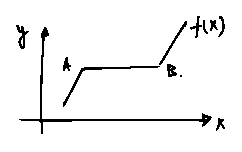
\includegraphics[scale=1.5]{figure.eps}
\end{center}
    
    \reason
    
    One only needs to see the slopes of the lines to know that at both $A$ and $B$, the rate of change \underline{before} the point 
    is different from the rate of change \underline{after} the point\newline 
    
    Hence, $f(x)$ is not differentiable at $A$ or $B$ \newline 
    
    Mathematically, we would say 
    \begin{align}
	\lim_{x\to A^-} f'(x) &\neq \lim_{x\to A^+} f'(x) \\
	\lim_{x\to B^-} f'(x) &\neq \lim_{x\to B^+} f'(x) 
\end{align}
\end{snippet} 
\end{document} 